\documentclass[../../main]{subfiles}
\begin{document}
\lstset{language=XML}

\section{robot modeling using URDF}
The Unified Robot Description Format (URDF) is an XML file format used to describe the physical properties of a robot in robotics applications, in particular within the Robot Operating System (ROS) ecosystem. It specifies the robot structure (links, joints, sensors and actuators etc.)

URDF can represent the kinematic and dynamic description of the robot, the visual
representation of the robot, and the collision model of the robot.
The following tags are the commonly used URDF tags to compose a URDF robot model:

\subsection{link:}\label{tags}
The link tag represents the single link of a robot. Using this tag, we can
model a robot link and its properties. The modeling includes the size, the shape,
and the color; it can even import a 3D mesh to represent the robot link. We can
also provide the dynamic properties of the link, such as the inertial matrix and the
collision properties.
The syntax is as follows:

\begin{codebox}[]{Defining a Robot Link in URDF}
  \begin{minted}{xml}
    <link name="<name of the link>">
        <inertial>...........</inertial>
        <visual> ............</visual>
        <collision>..........</collision>
    </link>
\end{minted}
  \end{codebox}
The following is a representation of a single link. The Visual section represents the
real link of the robot, and the area surrounding the real link is the Collision section.
The Collision section encapsulates the real link to detect a collision before hitting
the real link:
\begin{figure}[h]
\centering
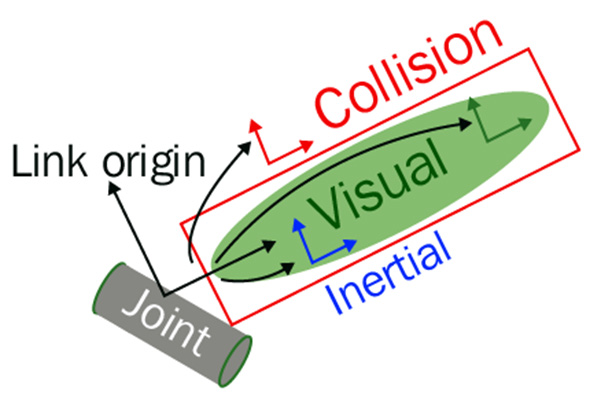
\includegraphics{sublatex/hashem/img/link1.jpg}
\caption{A visualization of the URDF link\cite{joseph2018mastering}}
\end{figure}

\subsection{joint:}
The \emph{joint} tag represents a robot joint. We can specify the kinematics and
dynamics of the joint and set the limits of the joint movement and its velocity. The
joint tag supports the different types of joints, such as \emph{revolute, continuous,
prismatic, fixed, floating,} and \emph{planar}.
The syntax is as follows:
\begin{codebox}[]{Defining a Robot joint in URDF}
  \begin{minted}{xml}
    <joint name="<name of the joint>">
    <parent link="link1"/>
    <child link="link2"/>
    <calibration .... />
    <dynamics damping = ..../>
    <limit effort = ..../>
    </joint>
\end{minted}
\end{codebox}
A URDF joint is formed between two links; the first is called the Parent link, and the
second is called the Child link. Note that a single joint can have a single parent and
multiple children at the same time. The following is an illustration of a joint and its links:
\begin{figure}[ht]
    \centering
    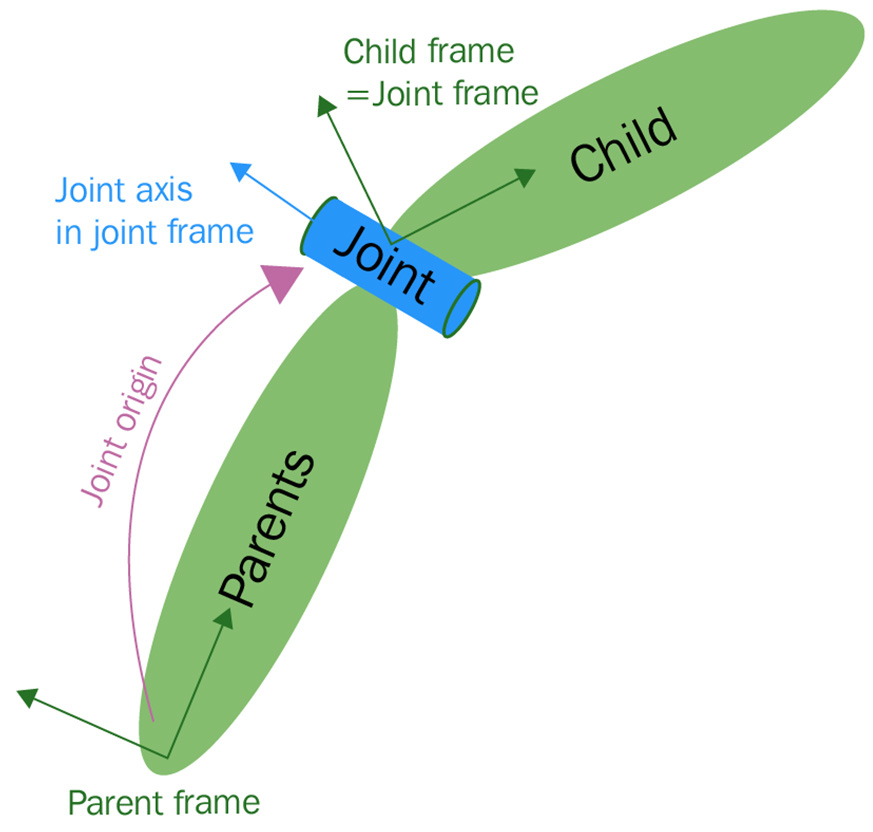
\includegraphics{sublatex/hashem/img/joint1.jpg}
    \caption{A visualization of the URDF joint\cite{joseph2018mastering}}
\end{figure}

\subsection{robot:}
This tag encapsulates the entire robot model that can be represented using
URDF. Inside the robot tag, we can define the name of the robot, the links, and the
joints of the robot.
The syntax is as follows:

\begin{codebox}[]{Defining a Robot Model in URDF}
  \begin{minted}{xml}
    <robot name="<name of the robot>">
    <link> ...... </link>
    <joint> ....... </joint>
    <joint> ........</joint>
    </robot>
\end{minted}
  \end{codebox}
A robot model consists of connected links and joints. Here is a visualization of the
robot model:
\begin{figure}[ht]
    \centering
    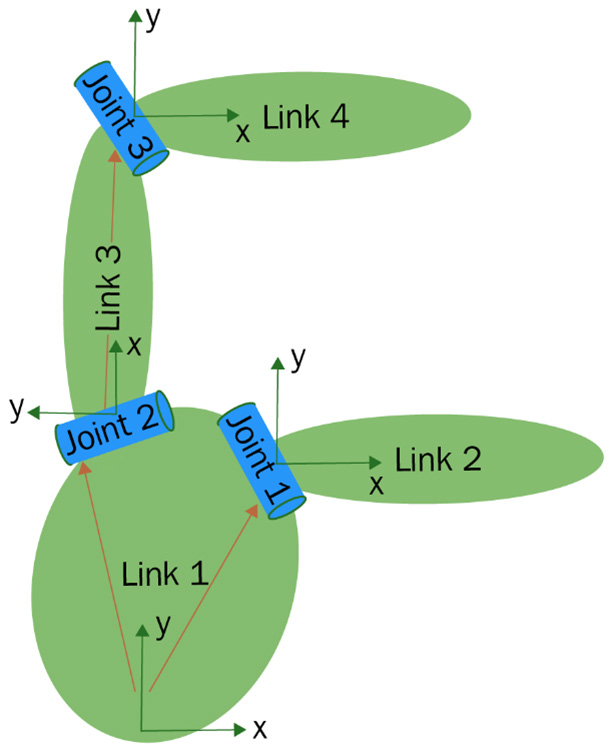
\includegraphics{sublatex/hashem/img/robot1.jpg}
    \caption{A visualization of a robot model with joints and links\cite{joseph2018mastering}}
\end{figure}

\subsection{gazebo:}
This tag is used when we include the simulation parameters of the
Gazebo simulator inside the URDF. We can use this tag to include gazebo plugins,
gazebo material properties, and more. The following shows an example that uses
gazebo tags:

\begin{codebox}[]{Defining Gazebo Material Properties in URDF }
  \begin{minted}{xml}
    <gazebo reference="link_1">
    <material>Gazebo/Black</material>
    </gazebo>
\end{minted}
  \end{codebox}
You can find more about URDF tags at \href{http://wiki.ros.org/urdf/XML}{wiki.ros}\cite{ros_urdf_xml}. We are now
ready to use the elements listed earlier to create a new robot from scratch. In the next
section, we are going to create a new ROS package containing a description of the different
robots.

\subsection{Adding physical and collision properties to a URDF model}
Before simulating a robot in a robot simulator, such as Gazebo or CoppeliaSim, we need
to define the robot link's physical properties, such as geometry, color, mass, and inertia, as
well as the collision properties of the link.
Good robot simulations can be obtained only if the robot dynamic parameters (for
instance, its mass, inertia, and more) are correctly specified in the urdf file. In the
following code, we include these parameters as part of the base\_link:
\begin{codebox}[]{Defining Physical and Collision Properties for a Robot Link in URDF}
  
  \begin{minted}{xml}
    <link name="base_link">
    ...
    <collision>
      <geometry>
          <box size="0.9 0.85 0.5"/>
      </geometry>
        <origin xyz="0.0 0.0 0.025" rpy="0.0 0.0 0.0"/>
    </collision>
    <inertial>
    <origin xyz="0 0 0" rpy="0 0 0"/>
    <mass value="35"/>
    <inertia ixx="3.2" ixy="0.0" ixz="0.0" iyy="4" iyz="0.0" izz="$3.9"/>
    </inertial>  </link>
\end{minted}
  \end{codebox}

\subsection{Transmission:}
\emph{transmission} tag is used to model the relationship between a robot's joints and actuators 
(such as motors, servos, or other mechanical devices that provide motion). 
It defines how power or motion is transferred from an actuator to a joint in the robot's structure.
The <transmission> tag usually works with <joint> and <actuator> tags to specify how an actuator controls the motion of the robot's joints:
\begin{codebox}[]{Modeling Joint-Actuator in URDF with "transmission"}
  \begin{minted}{xml}
    <robot name="example_robot">

    <!-- Define the joint -->
    <joint name="joint_1" type="revolute">
      <parent link="base_link"/>
      <child link="link_1"/>
      <axis xyz="0 0 1"/>
      <limit effort="10.0" velocity="1.0" lower="-1.57" upper="1.57"/>
    </joint>
    <!-- Define the transmission -->
    <transmission name="trans_1">
      <type>transmission_interface/SimpleTransmission</type>
      <joint name="joint_1"/>
      <actuator name="motor_1">
                     <!-- Gear ratio -->
        <mechanicalReduction>100.0</mechanicalReduction>
      </actuator>
    </transmission>
    <!-- Define the actuator (motor) -->
    <gazebo>
      <plugin name="motor_1_plugin" filename="libgazebo_motor_plugin.so">
        <motor_type>electric</motor_type>
        <max_power>100.0</max_power>
      </plugin>
    </gazebo>
  </robot>
\end{minted}
  \end{codebox}
\lstinline!<joint>!: The joint joint\_1 connects the base\_link to link\_1 and allows rotational movement. 
It has limits on effort and velocity.
\lstinline!<transmission>!: The transmission trans\_1 links joint\_1 to the actuator (motor motor\_1). It uses the SimpleTransmission type.
\lstinline!<mechanicalReduction>!: The actuator has a gear reduction of 100:1, meaning for every 100 rotations of the motor, the joint will rotate once.
\lstinline!<actuator>!: This specifies the motor (motor\_1) that will control joint\_1.
\lstinline!<gazebo>!: This block includes a Gazebo plugin (libgazebo\_motor\_plugin.so) to simulate the motor’s behavior in a Gazebo simulation environment, with specific motor properties like motor\_type and max\_power.

\subsection*{in summery:}

\renewcommand{\arraystretch}{1.4} % Increase row height for better readability
\begin{table}[ht]
    \centering
\begin{tcolorbox}[
    colback=red!5!white,colframe=red!75!black,
    title={\textbf{Dependencies for URDF Simulation in Gazebo}},
    fonttitle=\bfseries, coltitle=white, width=\linewidth
]

\centering
\begin{adjustbox}{max width=\linewidth} % Ensures the table fits within the page
\begin{tabular}{c|l|p{0.65\linewidth}} % Adjusted column width for better text wrapping
    
    \rowcolor{red!20} 
    \textbf{Step} & \textbf{Component} & \textbf{Effect if Missing} \\
    \midrule
    1 & Links (\texttt{<link>}) & The robot has no physical structure, making it impossible to define shapes, visualize, or interact with physics. \\
    2 & Joints (\texttt{<joint>}) & The robot will be completely rigid. No movement or articulation between parts is possible. \\
    3 & Inertia (\texttt{<inertial>}) & Gazebo will generate warnings or unstable behavior because the physics engine relies on mass and inertia properties to simulate motion correctly. \\
    4 & Collision (\texttt{<collision>}) & The robot will pass through objects and not interact with the environment physically. It may also affect contact-based sensors. \\
    5 & Gazebo Plugin (\texttt{<plugin>}) & The robot cannot interact with Gazebo’s physics, controllers, or sensors. Features like camera feeds, joint control, and custom physics will not work. \\
    6 & Gazebo Simulation & The robot cannot be tested in a realistic environment with physics, gravity, and other external forces. It remains a static model without dynamic behavior. \\
    7 & Transmission (\texttt{<transmission>}) & Motors will not work. Even if controllers are added, they will not be able to apply forces to move the joints. \\
\end{tabular}
\end{adjustbox}
\end{tcolorbox}
\caption{Essential Dependencies for Simulating a URDF in Gazebo}  % Caption outside the box
\end{table}
\newpage
\section{Creating URDF model}
After learning about URDF and its important tags, we can start some basic modeling
using URDF.
The robot’s URDF model comprises eight rigid links and seven joints,
designed to balance geometric simplicity with functional accuracy. 
The central chassis (base\_link), modeled as a rectangular prism, 
forms the structural foundation. 
Symmetrically attached to this base are two cylindrical wheels 
(left\_wheel, right\_wheel), each connected via continuous rotation 
joints to enable differential steering. A vertical lifting mechanism, 
represented as a cylinder (lifting\_mechanism), extends upward from the 
chassis through a prismatic joint, providing linear motion for height adjustment. 
Rigidly mounted atop this actuator is a box-shaped platform (platform), 
secured by a fixed joint to ensure stability. Three sensor units—two cameras 
(camera1, camera2) and a LiDAR (lidar)—are modeled as compact boxes and affixed 
to the platform through additional fixed joints, ensuring precise perceptual alignment. 
By prioritizing minimalistic shapes (cylinders for rotational elements, boxes for planar surfaces) 
and logical joint configurations (two continuous, one prismatic, and four fixed), the design achieves 
computational efficiency while retaining fidelity to the robot’s core mechanical and sensing capabilities.

\subsection{robot modeling using xacro}
The flexibility of URDF reduces when we work with complex robot models. Some of
the main features that URDF is missing include simplicity, reusability, modularity, and
programmability.
If someone wants to reuse a URDF block 10 times in their robot description, they can
copy and paste the block 10 times. If there is an option to use this code block and make
multiple copies with different settings, it will be very useful while creating the robot
description.
The URDF is a single file and we can't include other URDF files inside it. This reduces the
modular nature of the code. All code should be in a single file, which reduces the code's
simplicity.
Also, if there is some programmability, such as adding variables, constants, mathematical
expressions, and conditional statements in the description language, it will be more userfriendly.
Robot modeling using xacro meets all of these conditions. Some of the main features of
xacro are as follows:

\begin{itemize}
    \item \emph{Simplify URDF:} xacro is a cleaned-up version of URDF. It creates macros inside the robot description and reuses the macros. This can reduce the code length. Also, it can include macros from other files and make the code simpler, more readable, and more modular.
    \item \emph{Programmability:} The xacro language supports a simple programming statement in its description. There are variables, constants, mathematical expressions, conditional statements, and more that make the description more intelligent and efficient.
\end{itemize}

Instead of .urdf, we need to use the .xacro extension for xacro files.
Here is an explanation of the xacro code:
\begin{codebox}[]{XML Syntax with Xacro Extensions}
  \begin{minted}{xml}
    <?xml version="1.0"?>
    <robot xmlns:xacro="http://www.ros.org/wiki/xacro" name="my_robot">
\end{minted}
  \end{codebox}
These lines specify a namespace that is needed in all xacro files to parse the xacro file.
After specifying the namespace, we need to add the name of the xacro file. In the next section.

\subsection{Using properties}
Using xacro, we can declare constants or properties that are the named values inside the
xacro file, which can be used anywhere in the code. The main purpose of these constant
definitions is that instead of giving hardcoded values on links and joints, we can keep
constants, and it will be easier to change these values rather than finding the hardcoded
values and then replacing them.
An example of using properties is given here. We declare the length and radius of the
base link and the pan link. So, it will be easy to change the dimension here rather than
changing the values in each one:
\begin{codebox}[]{Xacro Properties to Define Reusable Values for Robot Dimensions}
  \begin{minted}{xml}
    <!-- body value -->
    <xacro:property name="base_length" value="0.9" />
    <xacro:property name="base_width" value="0.85" />
    <xacro:property name="base_hight" value="0.5" />
    <!-- Wheel values -->
    <xacro:property name="wheel_r" value="0.15" />
    <xacro:property name="wheel_length" value="0.05" />
    <!-- Lidar values  -->
    <xacro:property name="lidar_r" value="0.1" />
    <xacro:property name="lidar_l" value="0.05" />
\end{minted}
\end{codebox}

We can use the value of the variable by replacing the hardcoded value with the following
definition(\cref{xacro in urdf}):
\begin{codebox}[label=xacro in urdf]{}
  \begin{minted}{xml}
    <link name="base_link">
      <visual>
        <geometry>
          <box size="${base_length} ${base_width} ${base_hight}"/>
        </geometry>
          <origin xyz="0.0 0.0 ${base_hight/2.0}" rpy="0.0 0.0 0.0"/>
          <material name="green"/>
      </visual>
\end{minted}
  \end{codebox}

Here(\cref{xacro in urdf}), the value 0.9, is replaced with "{base\_length}", and "0.85" is
replaced with \\"{base\_width}".

\subsection{math expression in xacro}
We can build mathematical expressions inside \${} using basic operations such as +, -, *,
/, unary minus, and parentheses. Exponentiation and modulus are not supported yet. The
following is a simple math expression used inside the code:
\begin{codebox}[]{Math Expressions in Xacro}
  \begin{minted}{xml}
    <link name="platform_link">
    <visual>
      <geometry>
        <box size="${base_length/1.5} ${base_width/1.5} ${base_hight/8}"/>
      </geometry>
        <origin xyz="0.0 0.0 0" rpy="0.0 0.0 0.0"/>
        <material name="green"/>
    </visual>
\end{minted}
\end{codebox}

\subsection{xacro macros}
One of the main features of xacro is that it supports macros. We can use xacro to reduce
the length of complex definitions. Here is a xacro definition we used in our code to
specify inertial values,
\begin{codebox}[label=xacro macro]{Xacro Macros}
  \begin{minted}{xml}
    <xacro:macro name="box_inertia" params="m l w h xyz rpy">
    <inertial>
       <origin xyz="${xyz}" rpy="${rpy}"/>
       <mass value="${m}"/>
       <inertia ixx="${ (m/12)*(h*h + l*l) }" ixy="0.0" ixz="0.0" iyy="${(m/12)*(w*w + l*l)}" iyz="0.0" izz="${(m/12) * (w*w + h*h)}"/>
    </inertial>
   </xacro:macro>
\end{minted}
\end{codebox}
Here(\cref{xacro macro}), the macro is named box\_inertia, and its parameters are \{m ,l ,w ,h ,xyz ,rpy\}. we can pass these parameters as a vaues or as a xacro property(\cref{xacro macro result}):
\begin{codebox}[label=xacro macro result]{}
  \begin{minted}{xml}
<xacro:box_inertia m="5.0" l="${2*base_length}" w="${2*base_width}" h="${2*base_hight}" xyz="0.0 0.0 ${base_hight/2.0}" rpy="0.0 0.0 0.0"/>
\end{minted}
  \end{codebox}

\subsection{Including other xacro files}
We can extend the capabilities of the robot xacro by including the xacro definition of
sensors using the xacro:include tag. The following code snippet shows how to include
a sensor definition in the robot xacro:
\begin{codebox}[]{Including External Xacro Files to Extend Robot Model Definitions}
  \begin{minted}{xml}
<xacro:include filename="$(find ros_robot_pkg)/urdf/definition.xacro"/>
\end{minted}
  \end{codebox}
Here, we include a xacro file to call the definitions and the constants. 
\newpage
\section{Visualizing the 3D robot model in RViz}
After designing the URDF, we can view it on RViz.
We can create a launch file and put the following code into the launch folder:
\begin{codebox}[label=Rviz launch]{Launch File for Visualizing a 3D Robot Model in RViz}
  \begin{minted}{xml}
<launch>
<param name="robot_description" command="$(find xacro)/xacro $(find the_pkg_name)/.../my_robot.urdf.xacro" />
<node name="robot_state_publisher" pkg="robot_state_publisher" type="robot_state_publisher" />
<node name="rviz" pkg="rviz" type="rviz" args="-d $(find the_pkg_name)/rviz/config.rviz" />
<node name="joint_state_publisher" pkg="joint_state_publisher" 
type="joint_state_publisher"/>
<node name="joint_state_publisher_gui" pkg="joint_state_publisher_gui" type="joint_state_publisher_gui"/>
<!--  Controller Manager  -->
  <node name="controller_spawner" pkg="controller_manager" type="spawner" respawn="false" output="screen"
        args="diff_drive_controller" /> 
</launch>
    \end{minted}
  \end{codebox}
in \cref{Rviz launch} The \texttt{<launch>} tag is the root tag that defines the entire launch file. All the nodes and parameters that need to be launched are specified within this tag.

    The \texttt{<param>} tag sets the \texttt{robot\_description} parameter, which specifies the URDF or XACRO file that contains the robot’s description. In this case, the \texttt{command} attribute runs the \texttt{xacro} tool to process the \texttt{my\_robot.urdf.xacro} file located in the package specified by \texttt{the\_pkg\_name}.
    
    The \texttt{<node>} tag launches the \texttt{robot\_state\_publisher} node. This node reads the robot’s description and publishes the state of the robot (e.g., joint positions, transformations) to ROS topics. It uses the \texttt{robot\_description} parameter that was set earlier.
    
    The next \texttt{<node>} tag launches RViz, the visualization tool used to display the robot in a 3D environment. The \texttt{args} attribute specifies a pre-configured RViz setup file (\texttt{config.rviz}) located in the package \texttt{the\_pkg\_name}. This setup is used for visualizing the robot model and its movements.
    
    The subsequent \texttt{<node>} tags launch two joint state publisher nodes.\\ The \texttt{joint\_state\_publisher} node publishes the joint states (such as the positions of robot joints) to ROS topics. The \texttt{joint\_state\_publisher\_gui} node includes a graphical user interface (GUI) that allows users to interactively control the joint states of the robot.
    
    Finally, the \texttt{<node>} tag for the \texttt{controller\_spawner} node is responsible for spawning and managing robot controllers. The node is part of the \texttt{controller\_manager} package, and the \texttt{spawner} executable is used to spawn a controller, in this case, \texttt{diff\_drive\_controller}. The \texttt{respawn} attribute is set to \texttt{false}, so the node will not automatically respawn if it crashes. The \texttt{output} attribute ensures that the output from the node is printed to the screen.
    
    We can launch the model using the following command(\cref{launch rviz}):
    \begin{codebox}[label=launch rviz]{}
      \begin{minted}{bash}
        roslaunch the_pkg_name launch_file_name.launch
      \end{minted}
      \end{codebox}
    If everything works correctly, we will get the robot in RViz, as shown
    here(\cref{A visualization of a robot model with Rviz}):
    \begin{figure}[h!]
        \centering
        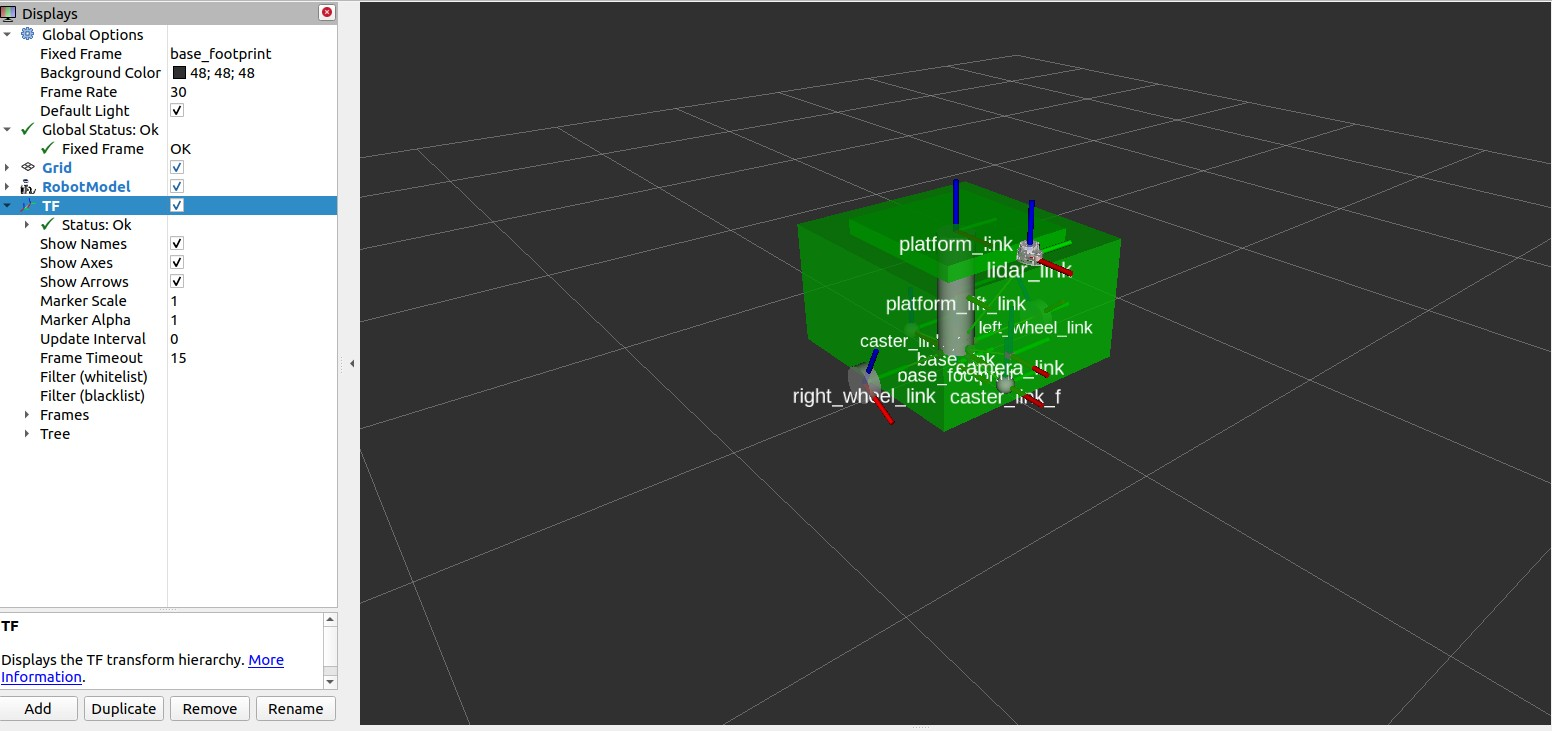
\includegraphics[width=\textwidth]{img/roborRvz1.jpg}
        \caption{A visualization of a robot model with Rviz}
\label{A visualization of a robot model with Rviz}
    \end{figure}
    \newpage
\subsection{Interacting with joints in Rviz}
In the previous version of ROS, the GUI of \texttt{joint\_state\_publisher} was enabled
thanks to a ROS parameter called \texttt{use\_gui}. To start the GUI in the launch file, this
parameter had to be set to true before starting the \texttt{joint\_state\_publisher} node.
In the current version of ROS, launch files should be updated to launch \texttt{joint\_state\_
publisher\_gui} instead of using \texttt{joint\_state\_publisher} with the \texttt{use\_gui}
parameter.

We can see that an extra GUI came along with RViz; it contains sliders to control the
Whell joints and the lifting platform joint. This GUI is called the Joint State Publisher Gui node and
belongs to the \texttt{joint\_state\_publisher\_gui} package:
\begin{codebox}[]{Joint State Publisher GUI in RViz}
  \begin{minted}{xml}
<node name="joint_state_publisher_gui" pkg="joint_state_
publisher_gui" type="joint_state_publisher_gui" />
\end{minted}
  \end{codebox}

We can include this node in the launch file using the following statement. The limits of
pan-and-tilt should be mentioned inside the joint tag:

\begin{codebox}[label=Prismatic Joint with Motion Limits in URDF for RViz Interaction]{Prismatic Joint with Motion Limits in URDF for RViz Interaction}
  \begin{minted}{xml}
<joint name="platform_lift_joint" type="prismatic">
    <origin xyz="0.0 0.0 ${base_hight / 2}" rpy="0.0 0.0 0.0"/>
    <parent link="base_link"/>
    <child link="platform_lift_link"/>
    <axis xyz="0 0 1"/> <!-- Movement along the Z-axis -->
    <!-- Motion range and limits -->
    <limit lower="0.0" upper="${base_hight/2}" effort="50" velocity="1.0"/> 
</joint>
\end{minted}
\end{codebox}
\newpage

In \cref{Prismatic Joint with Motion Limits in URDF for RViz Interaction} the \text{<limit>} tag defines the limits of effort, velocity, and angle. In this scenario,
effort is the maximum force supported by this joint, expressed in Newton; lower
and upper indicate the lower and upper limits of the joint, in radians for the revolute
joint and in meters for the prismatic joints. velocity is the maximum joint velocity
expressed in m/s.

The following screenshot shows the user interface that is used to interact with the robot
joints:
\begin{figure}[h]
    \centering
    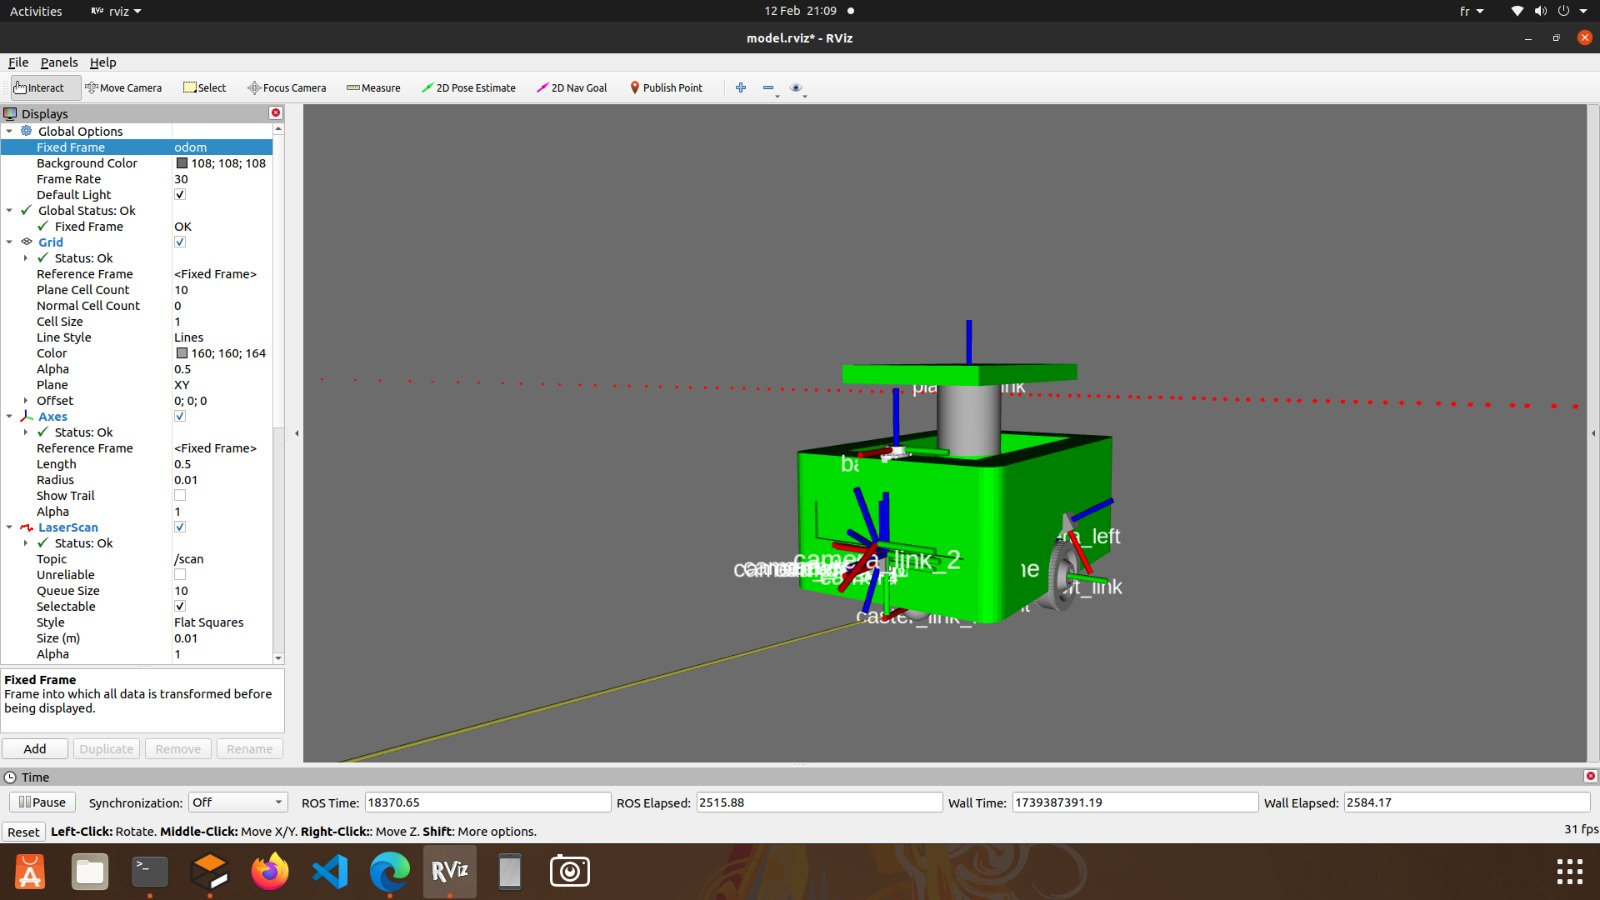
\includegraphics[width=\textwidth]{img/roborRvz.jpg}
    \caption{The joint level of the platform lifting mechanism}
    \end{figure}


    In this user interface, we can use the sliders to set the desired joint values. The basic
    elements of a urdf file have been discussed. In the next section, we will add additional
    physical elements to our robot model.

\end{document}












